\documentclass[letterpaper]{article}
\usepackage[margin=1in]{geometry}

\usepackage{float}
\usepackage{amsmath}
\usepackage{multicol}
\usepackage{listings}
\usepackage{tikz}
\usepackage[hidelinks]{hyperref}
\usetikzlibrary{calc, shapes, arrows}
\usetikzlibrary{automata,positioning} % For NFA

\tikzstyle{decision} = [diamond, draw, text centered, minimum height=2em]
\tikzstyle{process} = [rectangle, draw, text centered, minimum height=2em]
\tikzstyle{terminator} = [rectangle, draw, text centered, rounded corners, minimum height=2em]
\tikzstyle{data}=[trapezium, draw, text centered, trapezium left angle=60, trapezium right angle=120, minimum height=2em]
\tikzstyle{connector} = [draw, -latex']
\tikzstyle{curve} = [draw]

\usepackage{enumitem}
\usepackage{tcolorbox}

\renewcommand\thesection{\Alph{section}.}
\renewcommand\thesubsection{\arabic{subsection}.}
\renewcommand\thesubsubsection{\Roman{subsubsection}.}

% Remove Indentation
\usepackage{parskip}

\begin{document}

\begin{titlepage}
    \vspace*{\stretch{2.0}}
    \begin{center}
       \Large\textbf{Adaptable House: Anti-Sway} \\
       \Large\textbf{Official Control/Software Manual and Documentation} \\
       \vspace*{\stretch{10.0}}
       \large{Espinola, Malachi P} \\
       \large{Hokenstad, Ethan T} \\
       \large{Neff, Callen P} \\
       \large{Nguyen, Tri V} \\
       \large{Tevy, Vattanary} \\
       \vspace*{\stretch{1.0}}
       \Large{University of Washington} \\
       \Large{Department of Mechanical Engineering} \\
    \end{center}
\end{titlepage}

\newpage

\tableofcontents

\newpage

\section{Introduction}
\subsection{Project Motive}
The Adaptable House Capstone, begun by Mary Meyer, envisions an ``adaptable house" capable of helping patients with neuralmuscular disease, disorders, and injuries. The goal is for this house to assist people to walk around with a system that supports them, and adapts to their movements. The Anti-Sway division of this capstone was in charge of proving that lateral movement support could be provided to such users. Thus, at the Univeristy of Washington, the Anti-Sway Capstone group developed, tested and verified a small scale system that could prove that it can be done. 
\subsection{Manual Coverage}
A small and yet significant portion of this system is the embedded software that forms the cornerstone of the system by providing robust control for patients using the system. This document will thus provide a guide through, and for:
\begin{enumerate}
    \item Software Design of Existing System
    \item Implementation Decisions at Project Time
    \item Future Integration for Lift Control
\end{enumerate}
\subsection{Manual Limitations}
Although this manual aims to serve as a generous guide through the system, it should be noted that the subjects discussed are beyond trivial, and as such, one should be familiar with both control theory and common software development trends (the latter of which changes rapidly), although this manual will attempt to provide some background.

In particular, it is not a reiteration of every single software function ever defined. Such scrutinizing details are well documented within the code. This manual is here chiefly to explain any complicated algorithms, and the high level concepts captured by the software.

\newpage

\section{Requirements}
\subsection{Client-Side Requirements}
\subsection{Engineering Specifications}

\newpage

\section{Background}
\subsection{Introduction to Feedback Control}
\subsection{Finite State Machines}
\subsection{Software Design: Modularity}
\subsection{Parallelism and Mutual Exclusion}
\subsection{Microcomputers and C Programs}
\subsubsection{Error Codes}
\subsubsection{Memory Constraints}

\newpage
\section{Hardware Specifications}
\subsection{Microcomputer}
\subsubsection{MyRIO Wiring Connections}
\subsection{Mechanical Frame}
\subsubsection{Coordinate Axis Convention}

\section{Sensor/Actuator Specifications}
\subsection{Angle Sensing: Potentiometers}
\subsubsection{Iterations on Angle Sensing}
\subsection{Position Sensing: Encoders}
\subsection{Force Actuation: Motor}
\subsection{Velocity Actuation: Keypad}

\newpage

\section{Anti-Sway Control Modes and Schemes}
\subsection{Tracking Mode}
\subsection{Anti-Sway Mode}
\subsection{Force to Voltage Conversion}

\newpage

\section{Embedded Software} \label{section-emb-soft}
The following sections exclude discussion of \texttt{main.c}, which technically runs the program via its use of a main method. However, it is realtively simplistic, and simply calls on the system to start. The following sections will then discuss it.
\subsection{System Setup/Shutdown: \texttt{setup}}
This module is probably the simplest in concept. It is in charge of calling all modules' global startup and shutdown functions, which are one time only functions. The modules that depend on this are the MyRIO FPGA (\texttt{MyRio.h}), the Sensor/Actuator Module (\texttt{io.h}), and the data recording module (\texttt{record.h}), as shown in Figure \ref{setup-mdd}:
\begin{figure}[h]
    \centering
    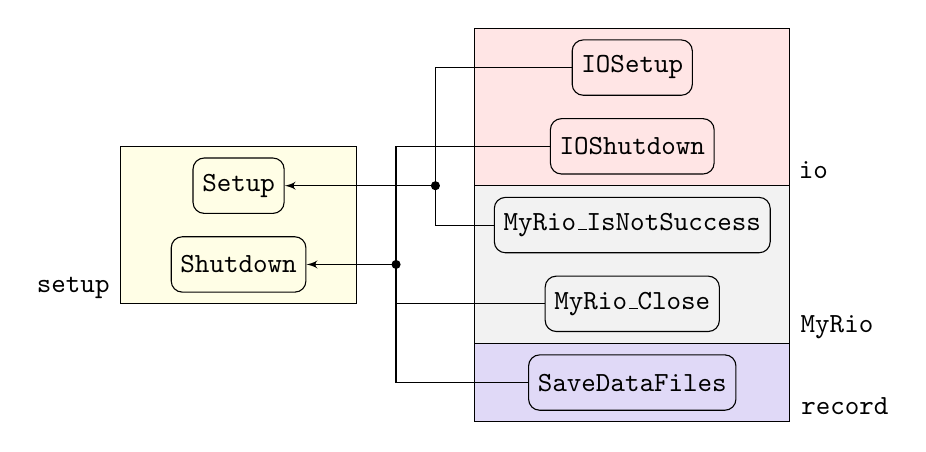
\begin{tikzpicture}
        
        \node[rectangle, draw, minimum width=3cm, minimum height=2cm, fill=yellow!10] (setup) at (-3, -1) {};
        \node at (-5.1, -1.8) {\texttt{setup}}; 
        \node[terminator] at (-3, -0.5) (Setup) {\texttt{Setup}};
        \node[terminator] at (-3, -1.5) (Shutdown) {\texttt{Shutdown}};
        
        \node[rectangle, draw, minimum width=4cm, minimum height=2cm, fill=red!10] (io) at (2, 0.5) {};
        \node at (4.3, -0.3) {\texttt{io}};
        \node[terminator] at (2, 1) (IOSetup) {\texttt{IOSetup}};
        \node[terminator] at (2, 0) (IOShutdown) {\texttt{IOShutdown}};
        
        \node[rectangle, draw, minimum width=4cm, minimum height=2cm, fill=gray!10] (MyRio) at (2, -1.5) {};
        \node at (4.6, -2.3) {\texttt{MyRio}};
        \node[terminator] at (2, -1) (MyRio_IsNotSuccess) {\texttt{MyRio\_IsNotSuccess}};
        \node[terminator] at (2, -2) (MyRio_Close) {\texttt{MyRio\_Close}};
        
        \node[rectangle, draw, minimum width=4cm, minimum height=1cm, fill=blue!80!red!15] (record) at (2, -3) {};
        \node at (4.7, -3.3) {\texttt{record}};
        \node[terminator] at (2, -3) (SaveDataFiles) {\texttt{SaveDataFiles}};

        \draw[connector] (IOSetup) -- (-0.5, 1) -- (-0.5, -0.5) -- (Setup);
        \draw[connector] (IOShutdown) -- (-1, 0) -- (-1, -1.5) -- (Shutdown);

        \draw[-] (MyRio_IsNotSuccess) -- (-0.5, -1) -- (-0.5, -0.5);
        \draw[-] (MyRio_Close) -- (-1, -2) -- (-1, -1.5);

        \draw[-] (SaveDataFiles) -- (-1, -3) -- (-1, -2);

        \filldraw[color=black] (-0.5, -0.5) circle (0.05);
        \filldraw[color=black] (-1, -1.5) circle (0.05);
        
    \end{tikzpicture}
    \caption{\texttt{setup} Module Dependency Diagram}
    \label{setup-mdd}
\end{figure}

It has two methods (both of which are \texttt{extern}):
\begin{enumerate}
    \item \texttt{int Setup()}: Starts the System
    \item \texttt{int Shutdown()}: Stops the System
\end{enumerate}
which both call the setup and shutdown functionality of the dependent modules, and return the conventional error code to signal if any of the dependent modules fail to initialize/deallocate. In particular, both methods start and stop:
\begin{enumerate}
    \item The ability to utilize the MyRio's FPGA (via \texttt{MyRio})
    \item The ability to interface with Sensors/Actuators (via \texttt{io})
    \item (For \texttt{Shutdown()} only) Writing all Data to MyRio's Disk (via \texttt{Record})
\end{enumerate}

It is also responsible for initializing the universal error code, which will be discussed later, but is an error signal shared accross threads with specific codes (somewhat related to the C construct of \texttt{errno}).

\subsubsection{Calibration: Setting up \texttt{io}}
Although it is strange to talk about another module within this context, talking about system initialization through \texttt{io} is appropriate here. The \texttt{io} module has to know what the reference position and angle are. To do so, it requests that the user set the trolley and the angle to the desired reference, and then sets it, all during the \texttt{IOSetup()} method. For reference, the displayed prompt is:

\begin{center}
    \begin{lstlisting}
        Please stablize for calibration.
        Press ENTR when ready._
    \end{lstlisting}
\end{center}
% \begin{tcolorbox}[colframe=red!75!black,colback=yellow!5, title=WARNING]
%     When you are trying this out, ensure that both the trolley and the rope/ball angle is completely still, or this will cause an inaccurate calibration.
% \end{tcolorbox}
More information about this particular method can be found in Section \ref{section-emb-soft}\ref{subsection-io} which will go into the specifics as to how exactly that is done.

\newpage

\subsection{System Management: \texttt{system}}
The \texttt{system} module is essentially responsible for running the entire software. It obviously does so by deffering basically each ``action'' to the other modules, so just like the \texttt{io} module, it does not really do a lot of heavy lifting. However, as the abstract representation of the system itself, it should be no surprise that its design resembles a Turing Machine (or a View/Controller, if you are familiar with the Model-View-Controller Software Design Pattern). Its interface is a simple function:
\begin{itemize}
    \item \texttt{int SystemExec()\footnote{Notice the \texttt{Exec} attached to the end of the name, which references the illusion that it is its own program and returns a conventional status code. This function does not actually clone the embedded process, its just a fun naming convention.}}: Executes the System
\end{itemize}
Now, we shall discuss how the system is structured on a high level. The following Finite State Automata, defined as a Nondeterministic Finite Automata (NFA)\footnote{This particular version of a Turing Machine is being invoked for simplicity, but also because the input to the \texttt{system} is quite literally a senary (base-6) string}, shows the state transitions for the System. Let us define the alphabet to be:
$$\boxed{A := \left\{1, 2, 3, 4, \leftarrow, E\right\}}$$
where $1-4$ are keypad keys, $\leftarrow$ is the keypad delete key, and $E$ is a universal error (with $\epsilon$ as the empty string/character). Then:
\begin{figure}[H]
    \centering
    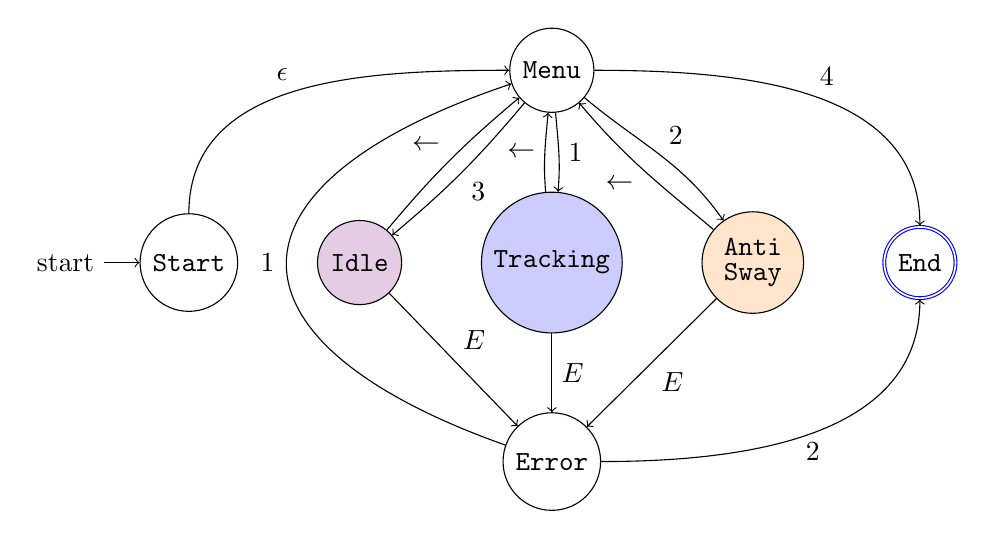
\begin{tikzpicture}
        \node[state, initial] (Start) {\texttt{Start}};
        \node[state, right =of Start, fill=violet!20] (Idle) {\texttt{Idle}};
        \node[state, right=of Idle, fill=blue!20] (Tracking) {\texttt{Tracking}};
        \node[state, right=of Tracking, fill=orange!20] (Anti-Sway) {\shortstack{\texttt{Anti}\\\texttt{Sway}}};
        \node[state, above =of Tracking] (Menu) {\texttt{Menu}};
        \node[state, below=of Tracking] (Error) {\texttt{Error}};
        \node[state, accepting, right= of Anti-Sway, draw=blue!100!black!100] (End) {\texttt{End}};

        \path[->]
        (Start) edge [out=90, in=180] node [above left] {$\epsilon$} (Menu)
        (Menu) edge [out=-130, in=40] node [below right] {$3$} (Idle)
               edge [out=-85, in=85] node [right] {$1$} (Tracking)
               edge [out=-40, in=125] node [above right] {$2$} (Anti-Sway)
        (Anti-Sway) edge [out=140, in=-50] node [below left] {$\leftarrow$} (Menu)
                    edge node [below right] {$E$} (Error)
        (Tracking) edge [out=95, in=-95] node [left] {$\leftarrow$} (Menu)
                   edge node [right] {$E$} (Error)
        (Idle) edge [out=50, in=-140] node [above left] {$\leftarrow$} (Menu)
               edge node [above right] {$E$} (Error)
        (Error) edge [out=0, in=270] node [below] {$2$} (End)
        (Menu) edge [out=0, in=90] node [above right] {$4$} (End);

        \node at (1, 0) {$1$};
        \draw[->] (Error) .. controls (0.3, -1) and (0.3, 1).. (Menu);
    \end{tikzpicture}
    \label{system-nfa}
    \caption{NFA for \texttt{system}}
\end{figure}
Note the correspondence of the 2 anti-sway modes with both the Tracking and Anti-Sway States. The presence of an idle mode is merely to check that sensors are working properly, it is not an actual control mode.

Implementing \texttt{system} becomes very straightforward from inspecting Figure \ref{system-nfa}. A function is assigned to each state, which are each responsible for indicating the next state to execute as well as executing the appropriate actions for that state, while all \texttt{SystemExec()} does is manage these states' execution flow. The dependency diagram for the \texttt{system} module is now shown in Figure \ref{system-mdd} (next page).
\begin{figure}[H]
    \centering
    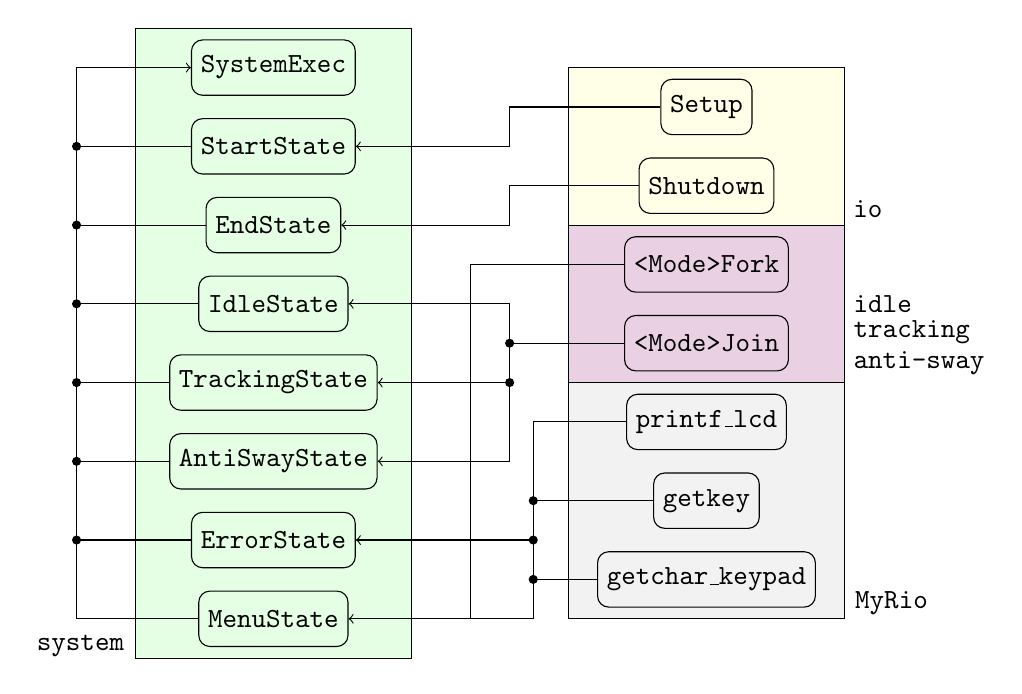
\begin{tikzpicture}

        \node[rectangle, draw, minimum width=3.5cm, minimum height=8cm, fill=green!10] at (0, -3.5) {};
        \node at (-2.45, -7.35) {\texttt{system}};
        \node[terminator] at (0, 0) (SystemExec) {\texttt{SystemExec}};
        \node[terminator] at (0, -1) (StartState) {\texttt{StartState}};
        \node[terminator] at (0, -2) (EndState) {\texttt{EndState}};
        \node[terminator] at (0, -3) (IdleState) {\texttt{IdleState}};
        \node[terminator] at (0, -4) (TrackingState) {\texttt{TrackingState}};
        \node[terminator] at (0, -5) (Anti-SwayState) {\texttt{AntiSwayState}};
        \node[terminator] at (0, -6) (ErrorState) {\texttt{ErrorState}};
        \node[terminator] at (0, -7) (MenuState) {\texttt{MenuState}};

        \node[rectangle, draw, minimum width=3.5cm, minimum height=2cm, fill=yellow!10] at (5.5, -1) {};
        \node at (7.55, -1.8) {\texttt{io}};
        \node[terminator] at (5.5, -0.5) (Setup) {\texttt{Setup}};
        \node[terminator] at (5.5, -1.5) (Shutdown) {\texttt{Shutdown}};

        \node[rectangle, draw, minimum width=3.5cm, minimum height=2cm, fill=blue!20!orange!20!violet!20] at (5.5, -3) {};
        \node at (8.2, -3.4) {\texttt{\shortstack[l]{\texttt{idle}\\\texttt{tracking}\\\texttt{anti-sway}}}};
        \node[terminator] at (5.5, -2.5) (ModeFork) {\texttt{<Mode>Fork}};
        \node[terminator] at (5.5, -3.5) (ModeJoin) {\texttt{<Mode>Join}};

        \node[rectangle, draw, minimum width=3.5cm, minimum height=3cm, fill=gray!10] at (5.5, -5.5) {};
        \node at (7.85, -6.8) {\texttt{MyRio}};
        \node[terminator] at (5.5, -4.5) (printf_lcd) {\texttt{printf\_lcd}};
        \node[terminator] at (5.5, -5.5) (getkey) {\texttt{getkey}};
        \node[terminator] at (5.5, -6.5) (getchar_keypad) {\texttt{getchar\_keypad}};

        \draw[->] (Setup) -- (3, -0.5) -- (3, -1) -- (StartState);
        \draw[->] (Shutdown) -- (3, -1.5) -- (3, -2) -- (EndState);
        \draw[->] (ModeFork) -- (2.5, -2.5) -- (2.5, -7) -- (MenuState);
        \draw[->] (ModeJoin) -- (3, -3.5) -- (3, -3) -- (IdleState);
        \draw[->] (3, -3.5) -- (3, -4) -- (TrackingState);
        \draw[->] (3, -4) -- (3, -5) -- (Anti-SwayState);
        \draw[->] (printf_lcd) -- (3.3, -4.5) -- (3.3, -6) -- (ErrorState);
        \draw[-] (3.3, -6) -- (3.3, -7) -- (2.5, -7);
        \draw[-] (getkey) -- (3.3, -5.5);
        \draw[-] (getchar_keypad) -- (3.3, -6.5);

        \draw[<-] (SystemExec) -- (-2.5, 0) -- (-2.5, -7) -- (MenuState);
        \draw[-] (-2.5, -1) -- (StartState);
        \draw[-] (-2.5, -2) -- (EndState);
        \draw[-] (-2.5, -3) -- (IdleState);
        \draw[-] (-2.5, -4) -- (TrackingState);
        \draw[-] (-2.5, -5) -- (Anti-SwayState);
        \draw[-] (-2.5, -6) -- (ErrorState);

        \filldraw[color=black] (3, -3.5) circle (0.05);
        \filldraw[color=black] (3, -4) circle (0.05);
        \filldraw[color=black] (3.3, -5.5) circle (0.05);
        \filldraw[color=black] (3.3, -6) circle (0.05);
        \filldraw[color=black] (3.3, -6.5) circle (0.05);

        \filldraw[color=black] (-2.5, -1) circle (0.05);
        \filldraw[color=black] (-2.5, -2) circle (0.05);
        \filldraw[color=black] (-2.5, -3) circle (0.05);
        \filldraw[color=black] (-2.5, -4) circle (0.05);
        \filldraw[color=black] (-2.5, -5) circle (0.05);
        \filldraw[color=black] (-2.5, -6) circle (0.05);

    \end{tikzpicture}
    \caption{\texttt{system} Module Dependency Diagram}
    \label{system-mdd}
\end{figure}

The description of such functions follows:
\begin{itemize}
    \item \texttt{static int StartState()}: Dedicated to setting up the System (by setting it up via \texttt{Setup()})
    \item \texttt{static int EndState()}: Dedicated to stopping the System (by shutting it down \texttt{Shutdown()})
    \item \texttt{static int IdleState(), TrackingState(), AntiSwayState()}: Runs the corresponding state, and exits them when $\leftarrow$ is pressed or a universal error occurs
    \item \texttt{static int ErrorState()}: Processes a universal error with user input
    \item \texttt{static int MenuState()}: Allows the user to choose any of the Modes, and navigates to it
\end{itemize}
To acomplish state execution and state transitions, the following data types are employed:
\begin{multicols}{2}
    \begin{center}
        \begin{lstlisting}[language=C]
            enum {
                ANTI_SWAY,
                TRACKING,
                IDLE,
                MENU,
                ERROR,
                START,
                END
            } state = START;
                \end{lstlisting}
    \end{center}
    
    \columnbreak
    \begin{center}
        \begin{lstlisting}[language=C]
        static int (* states[])()
            = {AntiSwayState,
                TrackingState,
                IdleState,
                MenuState,
                ErrorState,
                StartState,
                EndState};
            \end{lstlisting}
    \end{center}
\end{multicols}
Thus, any State Function can set the variable \texttt{state} using the \texttt{enum} constants, and all \texttt{SystemExec()} needs to do to continue execution flow is state the line: \texttt{states[state]()}.

\begin{tcolorbox}[colframe=blue!50!black!70,title=Future Modification]
    Notice it is very critical for these fields to align in both the \texttt{enum} and the \texttt{states} array, and for all functions in the array to have the exact same function signature (save the name of course).
\end{tcolorbox}

\newpage

\subsection{Sensor/Actuator Interfacing: \texttt{io}} \label{subsection-io}
\subsubsection{Smart Limits: Kinematic Limits}
\subsubsection{Keyboard: Multithreaded Resource Managament}
\subsection{Discrete Control: \texttt{discrete-lib}}
\subsubsection{Control Law Blocks: Control Made Easy}
\subsection{Modes: \texttt{idle}/\texttt{tracking}/\texttt{anti-sway}}
\subsubsection{Multiaxis Control}
\subsection{Thread Management: \texttt{thread-lib}}
\subsection{Data Requisition: \texttt{record}}
\subsection{Error Handling: \texttt{error}}
\subsubsection{Static Error Codes v.\texttt{errno}}

\newpage

\section{System Performance}
\subsection{Tracking Mode}
\subsection{Anti-Sway Mode}

\newpage

\section{Discussion}
\subsection{Encoder Connections}
\subsection{Better Data Acquisition}
\subsection{Gradient Descent: Controller Tuning}

\newpage

\section{Conclusion}

\newpage

\section{Appendix}
\subsection{Code Base}

\end{document}
